\section{Experiments}
\label{saber:sec:experiments}


\begin{table*}[!t]
\centering
\caption{
Quantitative results on the OpenS2V-Eval~\citep{yuan2025opens2v} benchmark.
Saber outperforms both closed-source and explicitly trained R2V methods, achieving the highest overall score in a zero-shot setting.
It also attains the best NexusScore for subject consistency and competitive performance on GmeScore and NaturalScore.
}
\resizebox{\linewidth}{!}{
\begin{tabular}{lcccccccc}
\toprule[1.5pt]
\textbf{Method} & \textbf{Total Score} $\uparrow$ & \textbf{Aesthetics} $\uparrow$ & \textbf{MotionSmoothness} $\uparrow$ & \textbf{MotionAmplitude} $\uparrow$ & \textbf{FaceSim} $\uparrow$ & \textbf{GmeScore} $\uparrow$ & \textbf{NexusScore} $\uparrow$ & \textbf{NaturalScore} $\uparrow$ \\
\midrule
\multicolumn{9}{c}{\cellcolor[HTML]{EFEFEF}\textit{Closed-source commercial R2V methods}} \\
Pika2.1~\citep{pika}                           & 51.88\%  & 46.88\% & 87.06\% & 24.71\% & 30.38\% & 69.19\% & 45.40\% & 63.32\% \\
Vidu2.0~\citep{vidu}                           & 51.95\%  & 41.48\% & 90.45\% & 13.52\% & 35.11\% & 67.57\% & 43.37\% & 65.88\% \\
Kling1.6~\citep{kling}                         & 56.23\%  & 44.59\% & 86.93\% & 41.60\% & 40.10\% & 66.20\% & 45.89\% & 74.59\% \\
\multicolumn{9}{c}{\cellcolor[HTML]{EFEFEF}\textit{Explicit R2V data-based training methods}} \\
SkyReels-A2~\citep{fei2025skyreels}            & 52.25\%  & 39.41\% & 87.93\% & 25.60\% & 45.95\% & 64.54\% & 43.75\% & 60.32\% \\
MAGREF~\citep{deng2025magref}                  & 52.51\%  & 45.02\% & 93.17\% & 21.81\% & 30.83\% & 70.47\% & 43.04\% & 66.90\% \\
Phantom-14B~\citep{liu2025phantom}             & 56.77\%  & 46.39\% & 96.31\% & 33.42\% & 51.46\% & 70.65\% & 37.43\% & 69.35\% \\
VACE-14B~\citep{jiang2025vace}                 & 57.55\%  & 47.21\% & 94.97\% & 15.02\% & 55.09\% & 67.27\% & 44.08\% & 67.04\% \\
BindWeave~\citep{li2025bindweave}              & 57.61\%  & 45.55\% & 95.90\% & 13.91\% & 53.71\% & 67.79\% & 46.84\% & 66.85\% \\
\multicolumn{9}{c}{\cellcolor[HTML]{EFEFEF}\textit{Zero-shot R2V methods}} \\
\textbf{Saber (Ours)}                          & \cellcolor[HTML]{CFE8D9}57.91\%  & 42.42\% & 96.12\% & 21.12\% & 49.89\% & 67.50\% & \cellcolor[HTML]{CFE8D9}47.22\% & 72.55\% \\
\bottomrule[1.5pt]
\end{tabular}
}
% \caption{
% \textbf{Quantitative results on the OpenS2V-Eval benchmark~\citep{yuan2025opens2v}.}
% Saber outperforms both closed-source and explicitly trained R2V methods, achieving the highest overall score in a zero-shot setting.
% It also attains the best NexusScore for subject consistency and competitive performance on GmeScore and NaturalScore.
% }
\label{saber:tab:opens2v_eval}
\end{table*}







\subsection{Datasets, Metrics and Implementation Details}

\noindent \textbf{Datasets.}
Benefiting from the masked training strategy, Saber is trained exclusively on video-text pair datasets, enabling the use of data from T2V and I2V sources.
Specifically, we employ the ShutterStock Video~\citep{sstk} dataset and generate captions for all video clips using Qwen2.5-VL-Instruct~\citep{bai2025qwen2}, thus constructing the corresponding video-text pairs for training.


\noindent \textbf{Metrics.}
To ensure fair comparison, we adopt the OpenS2V-Eval~\citep{yuan2025opens2v} benchmark and follow its official protocol for fine-grained evaluation of reference-to-video generation.
The benchmark contains 180 prompts across seven categories, spanning single-reference (face, human, entity) and multi-reference (multi-face, multi-human, human-entity) scenarios.
We report automated metrics where higher scores indicate better performance, including Aesthetics for visual quality, MotionSmoothness for temporal coherence, MotionAmplitude for motion magnitude, and FaceSim for identity preservation.
In addition, we use three OpenS2V-Eval metrics, NexusScore, NaturalScore, and GmeScore, which measure subject consistency, naturalness, and text-video alignment, respectively.


\noindent \textbf{Implementation Details.}
Saber is finetuned from the Wan2.1-14B~\citep{wan2025wan} model using our proposed masked training strategy on video-text pair datasets.
%
For the mask generator, we adopt a probabilistic sampling strategy for the foreground area ratio $r$: with 10\% probability, we set $r \in [0, 0.1]$ to simulate minimal and no reference information, enabling the model to handle varying numbers of reference images; with 80\% probability, we set $r \in [0.1,0.5]$ to represent typical primary subjects; and with the remaining 10\% probability, we set $r \in [0.5,1.0]$ to help the model learn from large reference images or background scenes.
%
For mask augmentation, we randomly apply rotation within $[-10, 10]$ degree, scaling in the range $[0.8, 2.0]$, horizontal flipping with 50\% probability, and shearing within $[-10, 10]$ degree.
We found these augmentations to be empirically effective at overcoming copy-paste artifacts.
%
We train our model with the objective defined in Eq.~\ref{eq:loss}, using the AdamW optimizer with $1e^{-5}$ learning rate and a global batch size of $64$.
During inference, we use BiRefNet~\citep{zheng2024bilateral} to segment the foreground subjects from the reference images.
Following the standard setting of Wan2.1~\citep{wan2025wan}, we generate videos with $50$ denoising steps and a CFG~\citep{ho2022classifier} guidance scale of $5.0$.


\subsection{Quantitative Results}

We follow \citet{yuan2025opens2v} and conduct a comprehensive evaluation on OpenS2V-Eval~\citep{yuan2025opens2v} benchmark, with the results presented in Tab.~\ref{saber:tab:opens2v_eval}.
The table compares three types of methods: closed-source commercial R2V methods, explicitly trained R2V methods, and our zero-shot R2V approach.
Compared with the closed-source commercial method Kling1.6~\citep{kling}, our model achieves a 1.68\% higher total score.
Among methods trained on explicit R2V datasets, our method surpasses Phantom~\citep{liu2025phantom} by 1.14\%, VACE~\citep{jiang2025vace} by 0.36\%, and BindWeave~\citep{li2025bindweave} by 0.30\%.
While these methods rely on costly explicit R2V datasets that are difficult to scale, our approach uses only text-video pairs with a masked training strategy, achieving the best overall performance in a zero-shot setting.

Among all sub-metrics, NexusScore best represents R2V performance by measuring subject consistency.
Saber achieves the highest NexusScore, exceeding Phantom by 9.79\%, VACE by 3.14\%, and BindWeave by 0.36\%.
This shows that the masked training strategy effectively learns subject features from video-text pairs in a zero-shot setting, outperforming all R2V-data-based models.
Our method also achieves competitive results on GmeScore (text-video alignment) and NaturalScore (video naturalness).



\begin{figure*}[t]
    \centering
    % \fbox{\rule{0pt}{8.5in} \rule{1.0\linewidth}{0pt}}
    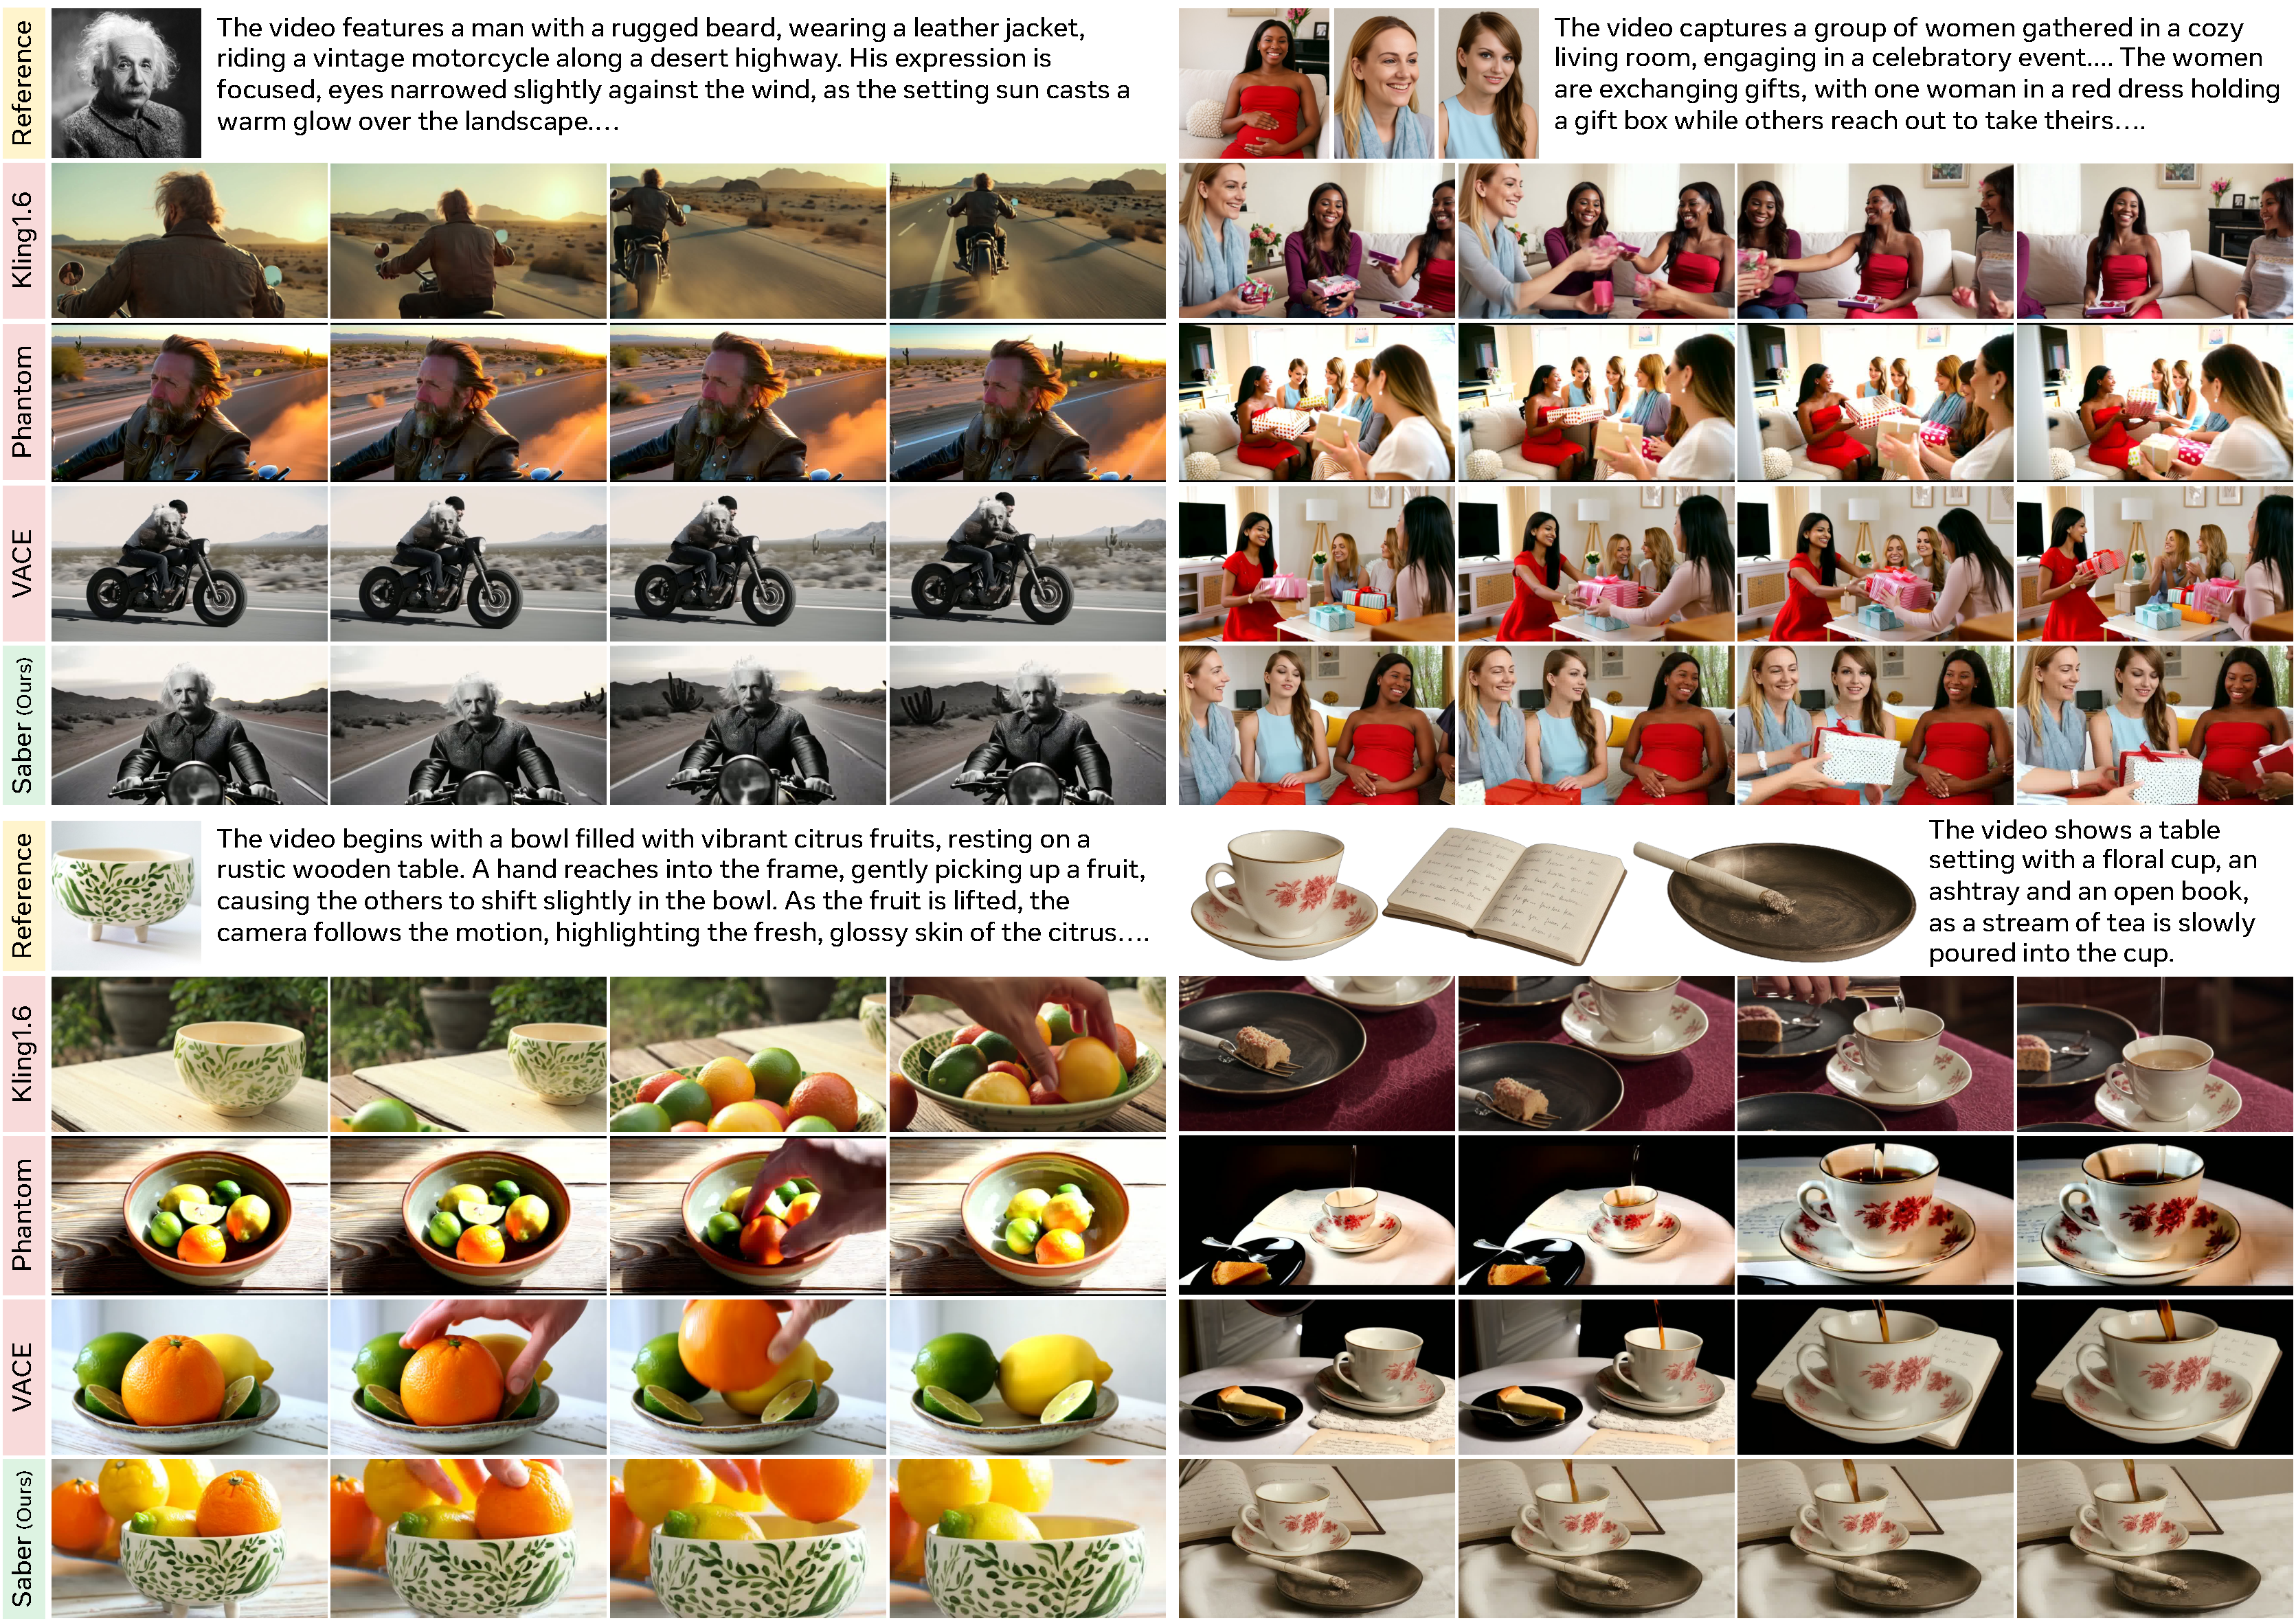
\includegraphics[width=1.0\linewidth]{Chapter7/Figures/visualization_opens2v_eval.pdf}
    \caption{
    Qualitative comparison with existing R2V methods.
    We compare Saber with Kling1.6~\citep{kling}, Phantom~\citep{liu2025phantom}, and VACE~\citep{jiang2025vace} across four scenarios: single/multiple human and object references.
    Saber accurately preserves subject identity and appearance, integrates multiple references coherently, and generates smoother, more visually consistent videos.
    }
    \label{saber:fig:vis_opens2v_eval}
\end{figure*}


\subsection{Qualitative Results}

We further conduct a qualitative comparison between Saber and existing methods, including Kling1.6~\citep{kling}, Phantom~\citep{liu2025phantom}, and VACE~\citep{jiang2025vace}. As shown in Fig.~\ref{saber:fig:vis_opens2v_eval}, we evaluate four scenarios with single/multiple human and object references.
i) In the top-left (single human reference), both Kling1.6 and Phantom fail to embed the reference subject into the generated video, leading to inconsistent facial appearances. VACE suffers from a copy-paste issue, directly overlaying the face from the reference image. In contrast, Saber generates a video with a consistent and text-aligned facial identity.
ii) In the bottom-left (single object reference), Kling1.6 produces a bowl with an incorrect leg structure, while Phantom and VACE fail to capture both the shape and appearance of the bowl from the reference. In contrast, our method, benefiting from the rich diversity of masked frames during masked training, accurately integrates the bowl's shape and appearance into the generated video.
iii) In the top-right (multiple human references), Kling1.6 embeds only one subject, Phantom duplicates the same identity twice, and VACE fails to inject facial information from the references. In contrast, Saber incorporates all three subjects and generates a coherent, natural video.
iv) In the bottom-right (multiple object references), Kling1.6 produces incorrect patterns on the cup, while Phantom and VACE generate correct cup textures but omit the ashtray, with VACE also showing temporal discontinuity. Saber, on the other hand, generates all referenced objects correctly and maintains smooth, consistent video quality.




% \subsection{User Study}


\subsection{Ablation Study}
We conduct a series of ablation studies to analyze the key components of Saber, including the masked training strategy, mask generator, mask augmentation, and attention mask in the attention mechanism.


\begin{table}[!t]
\centering
\caption{
Ablation study.
i) Masked training outperforms training on the OpenS2V-5M~\citep{yuan2025opens2v} (w/o masked training), demonstrating the advantage of the masked training strategy.
ii) Using only a single mask type reduces total score, while combining all types performs best, showing the importance of mask diversity.
iii) Fixing the foreground area ratio ($r=0.3$) leads to a further drop, indicating limited mask variation harms generalization.
}
\resizebox{0.7\linewidth}{!}{
\begin{tabular}{lcccccccc}
\toprule[1.5pt]
\textbf{Method} & \textbf{Total Score} $\uparrow$ & \textbf{GmeScore} $\uparrow$ & \textbf{NexusScore} $\uparrow$ & \textbf{NaturalScore} $\uparrow$ \\
\midrule
\textbf{Saber}                                 & 57.91\%  & 67.50\% & 47.22\% & 72.55\% \\
~~~w/o masked training                         & 56.24\%  & 67.27\% & 45.33\% & 70.19\% \\
~~~ellipse only                                & 54.56\%  & 67.98\% & 40.28\% & 72.54\% \\
~~~fourier only                                & 56.33\%  & 67.25\% & 44.82\% & 72.46\% \\
~~~polygon only                                & 56.49\%  & 67.41\% & 45.24\% & 72.21\% \\
~~~fixed $r=0.3$                               & 51.73\%  & 67.12\% & 39.20\% & 69.55\% \\
\bottomrule[1.5pt]
\end{tabular}
}
% \caption{
% \textbf{Ablation study.}
% Masked training outperforms training on the OpenS2V-5M~\citep{yuan2025opens2v} (w/o masked training), demonstrating the advantage of the masked training strategy.
% Using only a single mask type reduces total score, while combining all types performs best, showing the importance of mask diversity.
% Fixing the foreground area ratio ($r=0.3$) leads to a further drop, indicating limited mask variation harms generalization.
% }
\label{saber:tab:ablation_study}
\end{table}


\noindent \textbf{The Effect of Masked Training.}
To evaluate the effect of masked training, we finetune our model on the OpenS2V-5M~\citep{yuan2025opens2v} dataset using the same architecture.
As shown in Tab.~\ref{saber:tab:ablation_study}, masked training improves the total score by +1.67\%, indicating that it strengthens subject representation learning and reduces overfitting to specific reference cues.


\noindent \textbf{The Effect of Mask Generator.}
In Tab.~\ref{saber:tab:ablation_study}, we first analyze the mask type by training the model using only one type at a time.
Using only ellipse, Fourier, or polygon masks reduces total score by 3.35\%, 1.58\%, and 1.42\%, respectively, whereas combining all types yields the best results, showing that mask diversity is crucial for masked training.
We also fix the foreground area ratio $r$ to 0.3, which leads to a 6.18\% drop, indicating that restricting mask variation limits generalization.


\begin{figure}
    \centering
    % \fbox{\rule{0pt}{2in} \rule{1.0\linewidth}{0pt}}
    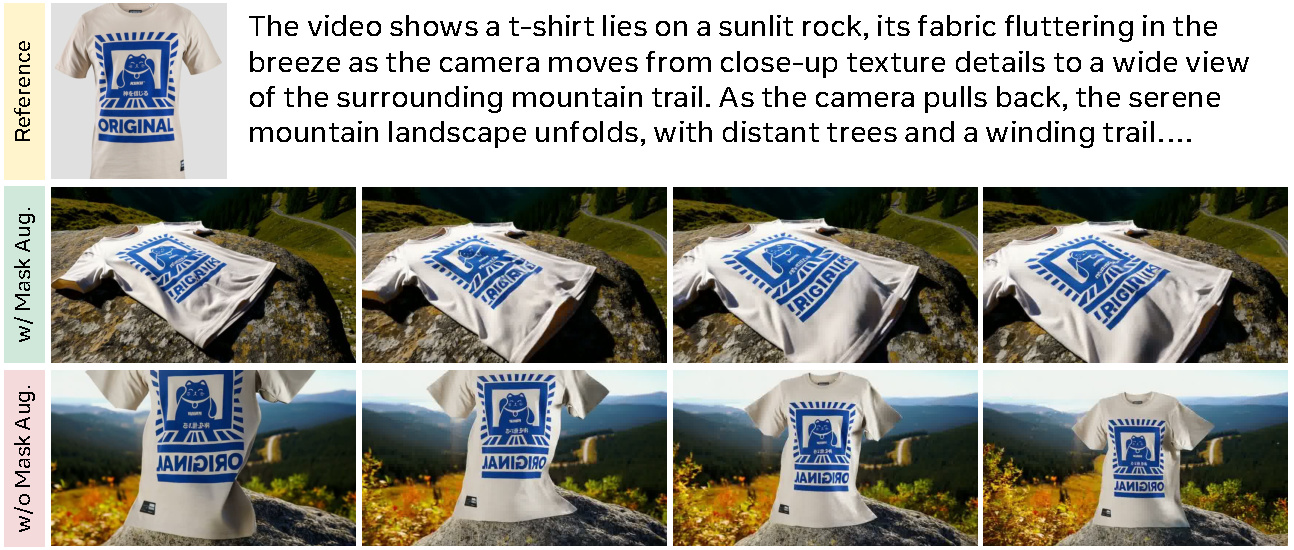
\includegraphics[width=0.5\linewidth]{Chapter7/Figures/ablation_mask_aug.pdf}
    \caption{
    Effect of mask augmentation.
    Without mask augmentation, the model shows copy-paste artifacts by directly copying reference content.
    Applying augmentation enables more natural and coherent video generation.
    }
    \label{saber:fig:ablation_mask_aug}
\end{figure}


\noindent \textbf{The Effect of Mask Augmentation.}
We evaluate the effect of mask augmentation by training the model with and without it. As shown in Fig.~\ref{saber:fig:ablation_mask_aug}, without augmentation, the model exhibits severe copy-paste artifacts, directly placing the T-shirt upright on the rock.
With augmentation (rotation, scaling, flipping, and shearing), the T-shirt naturally lies on the rock surface, resulting in more realistic and coherent compositions.
This demonstrates that geometric diversity in masking is crucial for natural video generation.





\noindent \textbf{The Effect of the Attention Mask.}
Finally, we examine the role of the attention mask in our attention mechanism, which constrains reference-video token interaction.
As shown in Fig.~\ref{saber:fig:ablation_attn_mask}, removing the attention mask introduces visible gray artifacts around the subject regions, as the model fails to correctly extract subjects from masked reference images (\eg, gray areas behind sunglasses or clocks). 
Incorporating the attention mask effectively resolves these issues, leading to cleaner subject separation, smoother blending, and improved overall video quality.


\begin{figure}[h]
    \centering
    % \fbox{\rule{0pt}{8.5in} \rule{1.0\linewidth}{0pt}}
    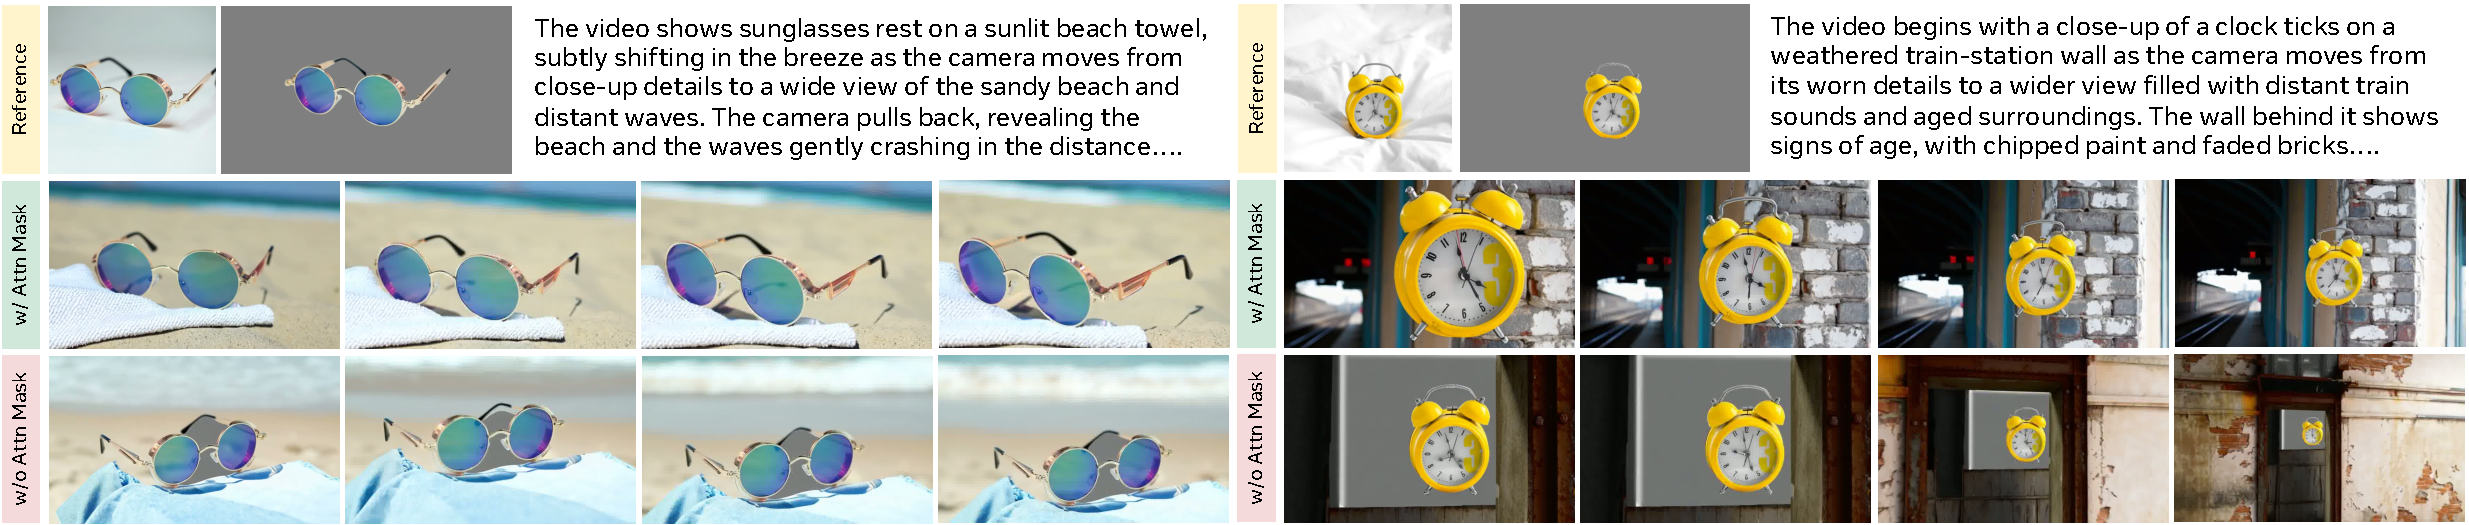
\includegraphics[width=1.0\linewidth]{Chapter7/Figures/ablation_attn_mask.pdf}
    \caption{
    Effect of the attention mask.
    Removing the attention mask introduces gray artifacts around subjects, while applying it ensures clean separation from the gray background and smoother, more natural video results.
    }
    \label{saber:fig:ablation_attn_mask}
\end{figure}




\subsection{Emergent Abilities}
In this section, we explore several interesting capabilities of Saber that emerged from its training strategy, demonstrating robustness beyond the standard R2V task.

% further evaluate Saber by verifying its ability to handle multiple reference images from either different subjects or different views of the same subject, and by assessing its cross-modal consistency between reference images and text prompts.



\begin{figure}
    \centering
    % \fbox{\rule{0pt}{8.5in} \rule{1.0\linewidth}{0pt}}
    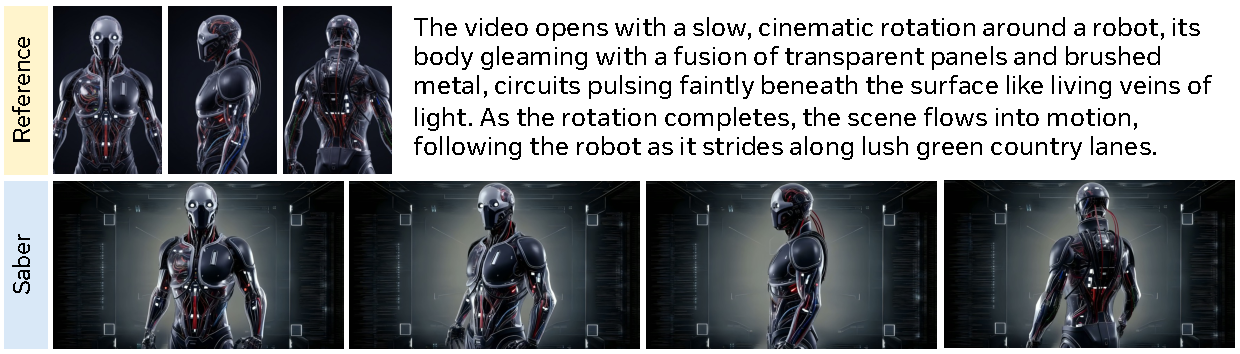
\includegraphics[width=0.5\linewidth]{Chapter7/Figures/one_subject_multi_view.pdf}
    \caption{
    Qualitative results on multiple reference images of the same subject.
    Given the front, side, and back views of a robot as reference, Saber correctly recognizes them as the same subject and integrates multi-view appearance features into a coherent video, accurately preserving fine structural and surface details.
    }
    \label{saber:fig:one_subject_multi_view}
\end{figure}



\noindent \textbf{Single Subject Multiple Views.}
% In the multiple reference images scenario shown in Fig.~\ref{saber:fig:vis_opens2v_eval}, each reference image represents a different subject.
We test Saber's ability to handle multiple reference images corresponding to different views of the same subject.
As shown in Fig.~\ref{saber:fig:one_subject_multi_view}, we use the front, side, and back views of a robot as reference inputs to Saber.
The results show that Saber successfully understands that all reference images depict the same subject (the robot) and integrates the appearance feature from different views into a single coherent video subject.
Despite the robot's complex surface details and wiring structure, Saber accurately captures and synthesizes these visual characteristics into the generated video.



\begin{figure}[h]
    \centering
    % \fbox{\rule{0pt}{8.5in} \rule{1.0\linewidth}{0pt}}
    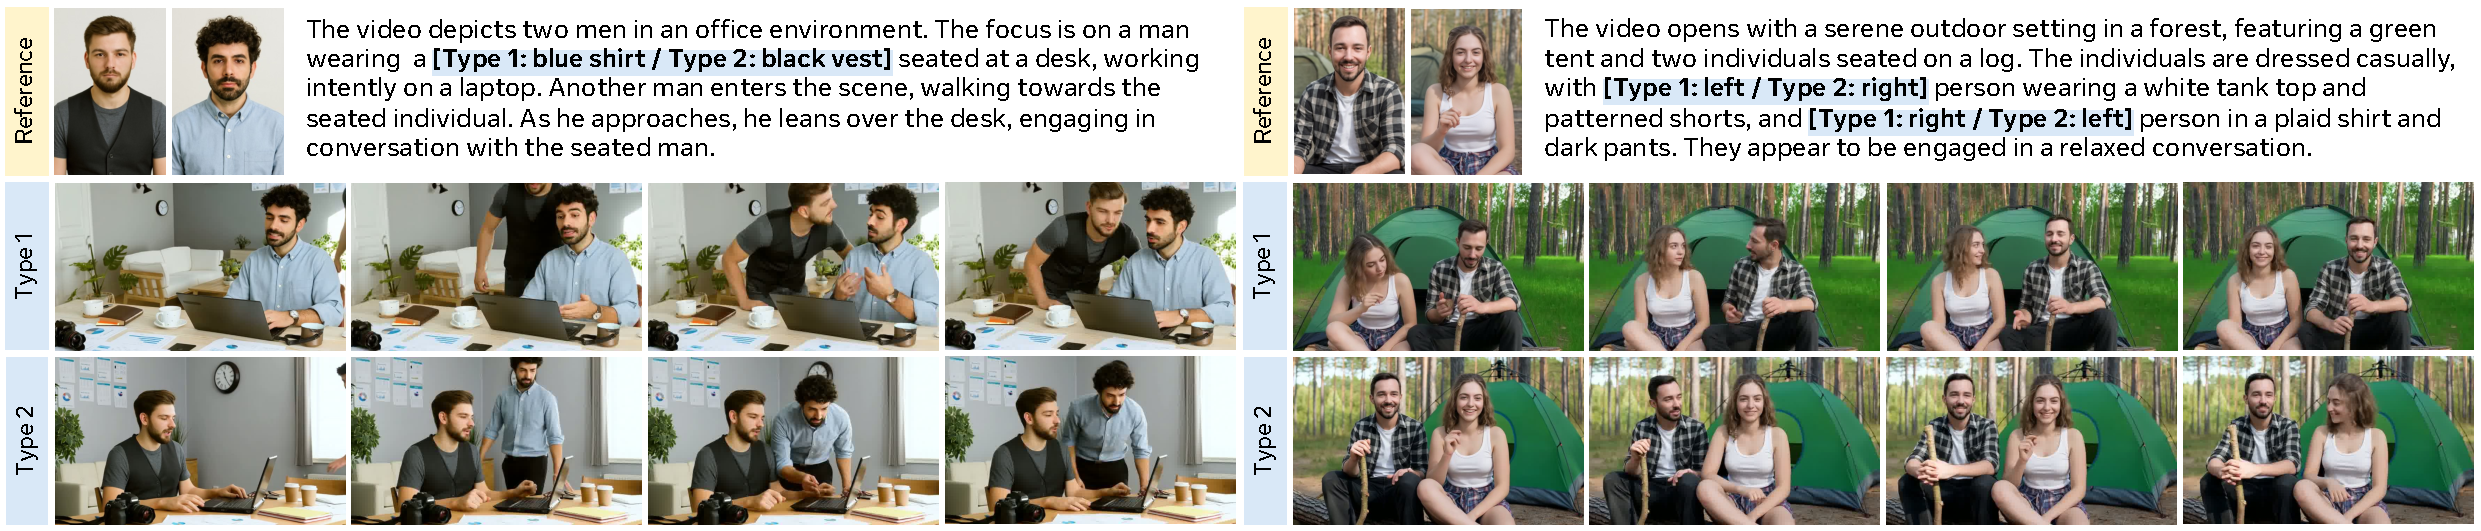
\includegraphics[width=1.0\linewidth]{Chapter7/Figures/cross_modal_alignment.pdf}
    \caption{
    Qualitative results of cross-modal alignment between reference images and text prompts.
    By swapping subject descriptions in the prompts (\eg, clothing color or subject positions), Saber accurately reflects the corresponding visual changes, demonstrating robust alignment between reference images and textual descriptions through its attention mechanisms.
    }
    \label{saber:fig:cross_modal_alignment}
\end{figure}

\noindent \textbf{Cross-Modal Alignment.}
We also evaluate the model's alignment between reference images and text prompts by swapping subject descriptions and observing the corresponding video changes.
As shown in Fig.~\ref{saber:fig:cross_modal_alignment}, when altering prompts such as ``a man wearing a blue shirt seated'' (Type~1) and ``a man wearing a black vest seated'' (Type~2), Saber correctly aligns subjects with their descriptions.
Similarly, when swapping the positions of a man and woman in the second case, the model accurately reflects the change.
This demonstrates that, as described in Sec.~\ref{saber:sec:model_design}, the interaction between video and reference tokens through self-attention, followed by cross-attention with text prompt features, enables robust reference image-text alignment.
